\section{Teori}
I boken ''Software Product Quality Control'' \cite{SPQC} nämns ett antal definitioner som förtydligör vad kvalitetssäkring innebär, dessa syns nedan.  

\begin{itemize}
  \item Quality assurance: a planned and systematic pattern of all actions necessary to provide adequate confidence that an item or product conforms to established technical requirements. 
  \item Constructive quality assurance: All means to be used in constructing a product in a way so it  meets its quality requirements. 
  \item Analyctical quality assurance: All means of analysing the state of the quality of a product. 
\end{itemize}
\noindent Kvalitetssäkring innebär följaktligen att man som leverantör av en produkt eller tjänst ska se till att de uppfyller de krav som har satts upp i en eventuell kravspecifikation. Att man under arbetsgången analyserar om man är på väg att uppfylla kraven eller inte, isåfall måste detta åtgärdas omedelbart.
\newline
\newline
Med detta sagt finns det flera steg i ett projekt att kvalitetssäkra. Ett effektivt sätt att göra detta på är genom att följa Shewhart cykeln, det vill säga planera, göra, studera och agera (PGSA).
\newline
\centerline{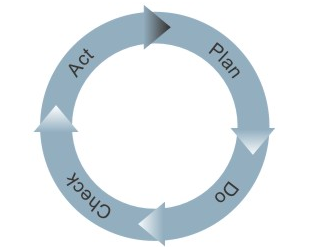
\includegraphics[scale=0.5]{ruben-tex/graphic/shewhartcycle}}


